\pdfminorversion=4
\documentclass[aspectratio=169]{beamer}

\mode<presentation>
{
  \usetheme{default}
  \usecolortheme{default}
  \usefonttheme{default}
  \setbeamertemplate{navigation symbols}{}
  \setbeamertemplate{caption}[numbered]
  \setbeamertemplate{footline}[frame number]  % or "page number"
  \setbeamercolor{frametitle}{fg=white}
  \setbeamercolor{footline}{fg=black}
} 

\usepackage[english]{babel}
\usepackage[utf8x]{inputenc}
\usepackage{tikz}
\usepackage{courier}
\usepackage{array}
\usepackage{bold-extra}
\usepackage{minted}
\usepackage[thicklines]{cancel}
\usepackage{fancyvrb}

\xdefinecolor{dianablue}{rgb}{0.18,0.24,0.31}
\xdefinecolor{darkblue}{rgb}{0.1,0.1,0.7}
\xdefinecolor{darkgreen}{rgb}{0,0.5,0}
\xdefinecolor{darkgrey}{rgb}{0.35,0.35,0.35}
\xdefinecolor{darkorange}{rgb}{0.8,0.5,0}
\xdefinecolor{darkred}{rgb}{0.7,0,0}
\definecolor{darkgreen}{rgb}{0,0.6,0}
\definecolor{mauve}{rgb}{0.58,0,0.82}

\title[2021-07-14-scipy-awkward-for-3-minutes]{\mbox{
\includegraphics[width=6 cm]{awkward-logo.pdf}}\vspace{-0.5 cm}}
\author{Jim Pivarski}
\institute{Princeton University -- IRIS-HEP}
\date{July 14, 2021}

\usetikzlibrary{shapes.callouts}

\begin{document}

\logo{\pgfputat{\pgfxy(0.11, 7.4)}{\pgfbox[right,base]{\tikz{\filldraw[fill=dianablue, draw=none] (0 cm, 0 cm) rectangle (50 cm, 1 cm);}\mbox{\hspace{-8 cm}
\includegraphics[height=1 cm]{princeton-logo-long.png}\hspace{0.1 cm}\raisebox{0.1 cm}{
\includegraphics[height=0.8 cm]{iris-hep-logo-long.png}}\hspace{0.1 cm}}}}}

\begin{frame}
  \vspace{0.45 cm}
  \titlepage
\end{frame}

\logo{\pgfputat{\pgfxy(0.11, 7.4)}{\pgfbox[right,base]{\tikz{\filldraw[fill=dianablue, draw=none] (0 cm, 0 cm) rectangle (50 cm, 1 cm);}\mbox{\hspace{-8 cm}
\includegraphics[height=1 cm]{princeton-logo.png}\hspace{0.1 cm}\raisebox{0.1 cm}{
\includegraphics[height=0.8 cm]{iris-hep-logo.png}}\hspace{0.1 cm}}}}}

% Uncomment these lines for an automatically generated outline.
%\begin{frame}{Outline}
%  \tableofcontents
%\end{frame}

% START START START START START START START START START START START START START

\begin{frame}{Awkward Array: NumPy-like idioms on JSON-like data}
\vspace{0.15 cm}
\begin{columns}
\column{1.1\linewidth}
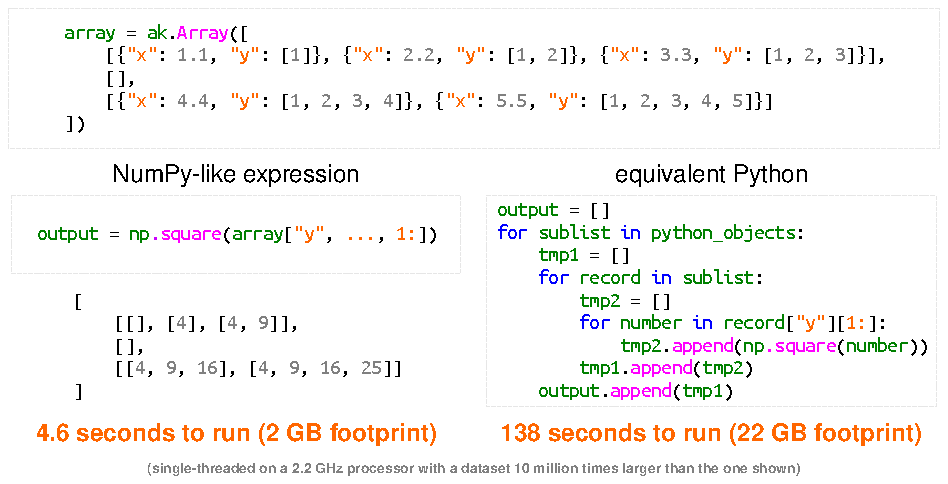
\includegraphics[width=\linewidth]{pivarski-one-slide-summary.pdf}
\end{columns}
\end{frame}

\begin{frame}[fragile]{Extended example: histogram of intervals in Million Song Dataset}
\vspace{0.2 cm}
\scriptsize
\begin{minted}{python}
import awkward as ak, numpy as np

# read an 80 GB Parquet dataset as a lazy array (through pyarrow)
millionsongs = ak.from_parquet("s3://pivarski-princeton/millionsongs/", lazy=True)

# volume of each half-step pitch (0-11) in each quarter-second segment of each song
pitches = millionsongs.analysis.segments.pitches
# <Array [[[0.294, 0.158, ... 0.083, 1, 0.078]]] type='1000000 * var * var * float64'>

# loudest pitch in each segment (axis=-1 applies to the deepest level of nesting)
loudest_pitches = ak.argmax(pitches, axis=-1)

# change in loudest-pitch from each segment to the next (list lengths vary with song)
intervals = loudest_pitches[:, 1:] - loudest_pitches[:, :-1]

# not including zero change (extremely variable)
nonzero_intervals = intervals[intervals != 0]

# histogram them
np.histogram(
    np.asarray(ak.flatten(nonzero_intervals)),
    bins=np.arange(-11.5, 12.5),
)
\end{minted}

\vspace{-2.85 cm}
\hfill 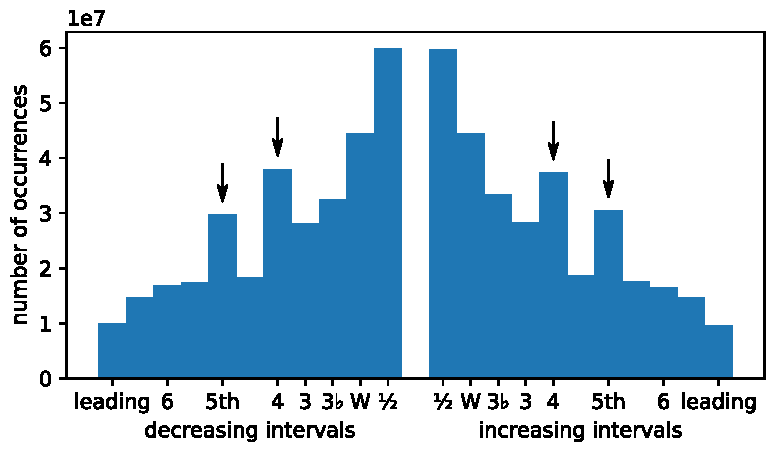
\includegraphics[width=0.4\linewidth]{million-song-histogram.pdf}
\end{frame}

\begin{frame}[fragile]{Extended example: same thing in Numba}
\vspace{0.2 cm}
\scriptsize
\begin{minted}{python}
import awkward as ak, numpy as np, numba as nb

millionsongs = ak.from_parquet("s3://pivarski-princeton/millionsongs/", lazy=True)

@nb.jit
def collect_pitch_intervals(millionsongs):
    pitch_intervals = np.zeros(23, np.int64)     # histogram as an array to fill

    for song in millionsongs:                    # iteration over variable-length songs
        previous = None

        for segment in song.analysis.segments:   # iteration over segments
            loudest_pitch = np.argmax(np.asarray(segment.pitches))

            if previous is not None:
                interval = loudest_pitch - previous
                if interval != 0:
                    pitch_intervals[interval + 11] += 1
            previous = loudest_pitch

    return pitch_intervals

collect_pitch_intervals(millionsongs)   # compiled by Numba, including lazy array
\end{minted}
\end{frame}

\begin{frame}{Actively extending beyond its original domain (particle physics)}
\large
\vspace{0.35 cm}
\textcolor{darkorange}{\bf Variable-length, nested data is a common problem,} so Awkward Array is a general-purpose library: working with nested lists, records, and missing data.

\vspace{0.35 cm}
But scientists in different fields have revealed gaps in scope:

\begin{itemize}
\item Radio astronomers asked for complex numbers: \mbox{\normalsize \href{https://github.com/scikit-hep/awkward-1.0/issues/392}{\textcolor{blue}{\#392}}, \href{https://github.com/scikit-hep/awkward-1.0/pull/421}{\textcolor{blue}{\#421}}, \href{https://github.com/scikit-hep/awkward-1.0/pull/652}{\textcolor{blue}{\#652}}, \href{https://github.com/scikit-hep/awkward-1.0/issues/857}{\textcolor{blue}{\#857}}, \href{https://github.com/scikit-hep/awkward-1.0/pull/858}{\textcolor{blue}{\#858}}\hspace{-0.5 cm}}
\item Data scientists asked for date-times: {\normalsize \href{https://github.com/scikit-hep/awkward-1.0/issues/913}{\textcolor{blue}{\#913}}, \href{https://github.com/scikit-hep/awkward-1.0/pull/911}{\textcolor{blue}{\#911}}, \href{https://github.com/scikit-hep/awkward-1.0/issues/909}{\textcolor{blue}{\#909}}, \href{https://github.com/scikit-hep/awkward-1.0/pull/835}{\textcolor{blue}{\#835}}, \href{https://github.com/scikit-hep/awkward-1.0/issues/367}{\textcolor{blue}{\#367}}}
\end{itemize}

\vspace{0.35 cm}
Starting a 3-year project {\normalsize (\href{https://www.nsf.gov/awardsearch/showAward?AWD_ID=2103945&HistoricalAwards=false}{\textcolor{blue}{NSF OAC-2103945}})} to ensure that Awkward Array works for use-cases across the sciences. {\normalsize (Note: \href{https://puwebp.princeton.edu/AcadHire/apply/application.xhtml?listingId=21021}{\textcolor{blue}{postdoc opportunity}}.)}

\vspace{0.35 cm}
\setlength{\fboxsep}{0.3 cm}
\fbox{\begin{minipage}{0.95\linewidth}We're actively seeking collaborations with scientists and data scientists with ``awkward'' data problems, to ensure that Awkward Array addresses them.\end{minipage}}

\normalsize
\vspace{0.35 cm}
Especially if this will lead to better integration with other scientific Python libraries and GPUs. (Dask integration and full GPU support are major parts of this project.)
\end{frame}

\begin{frame}{What's been happening recently?}
Since \href{https://youtu.be/WlnUF3LRBj4}{last year's introductory presentation}, Awkward Array
\begin{itemize}
\item released version 1.0 (Dec 5, 2020) and adopted bimonthly releases (now 1.4)
\item merged 346 PRs from 18 contributors: 4 undergrads, 2 engineers, 12 ``external''
\item $\sim$30,000 pip downloads/month (mostly physicists)
\end{itemize}
\begin{itemize}
\item Sorting (all \mintinline{python}{axis} depths), lexicographic for strings
\item Parquet input/output, including lazy reading
\item Refactoring some C++ infrastructure to Python for better Python integration
\end{itemize}

\end{frame}


\end{document}
